%%%%%%%%%%%%%%%%%%%%%%%%%
%                          %
% ----- INTRODUCTION ----- %
%                          %
%%%%%%%%%%%%%%%%%%%%%%%%%%

\section{Analyse}

	\subsection{Données de l'étude de Kosinski}

		\subsubsection{Introduction}

			Michal Kosinski se présente sur son site web\cite{michal-kosinski} comme un "psychologist and data scientist". L'étude qu'il a co-rédigée à l'Université de Stanford en 2016 a eu un impact important sur le monde académique et même industriel, en montrant les possibilités techniques ouvertes par la récolte de données simples d'utilisateurs : les "likes" Facebbok.

			Ainsi, il est montré qu'avec un peu plus de 300 "likes" tirés une personne, il est possible de définir avec une précision remarquable (mieux que son époux/épouse) des traits psychologiques, ainsi que d'autres caractéristiques personnelles.

		\subsubsection{Résumé}

			Une enquête a été menée auprès d'une population variée de personnes possédant un compte Facebook. Les données concernant leurs "likes" ont été récoltées, ainsi que des données personnelles pouvant être disponible (ou non) selon le souhait de l'utilisateur sur Facebook, comme ses informations démographiques. Des tests psychologiques ont été également réalisés par une certaine partie des utilisateurs afin de pouvoir trouver des corrélations entre les pages likées et certains trraits psychologiques.

			Cette enquête a rencontré un succès très large, et le nombre de personne ayant répondu à l'enquête, au moins en partie, se compte en millions.

			Les résultats présentés à la fin de l'étude sont inattendus : Michal annonce qu'il est possible de prédire certains comportements d'une personne mieux que son entourage le plus proche.

			Un des modèles crées avec les données récoltées, permet d'estimer le profil psychologique d'un participant selon cinq axes différents, en se basant sur ses likes Facebook. La figure~\ref{a-talk1} montre la précision obtenue par le modèle en fonction du nombre de likes utilisé en entrée.

			\begin{figure}[ht]
				\centering
				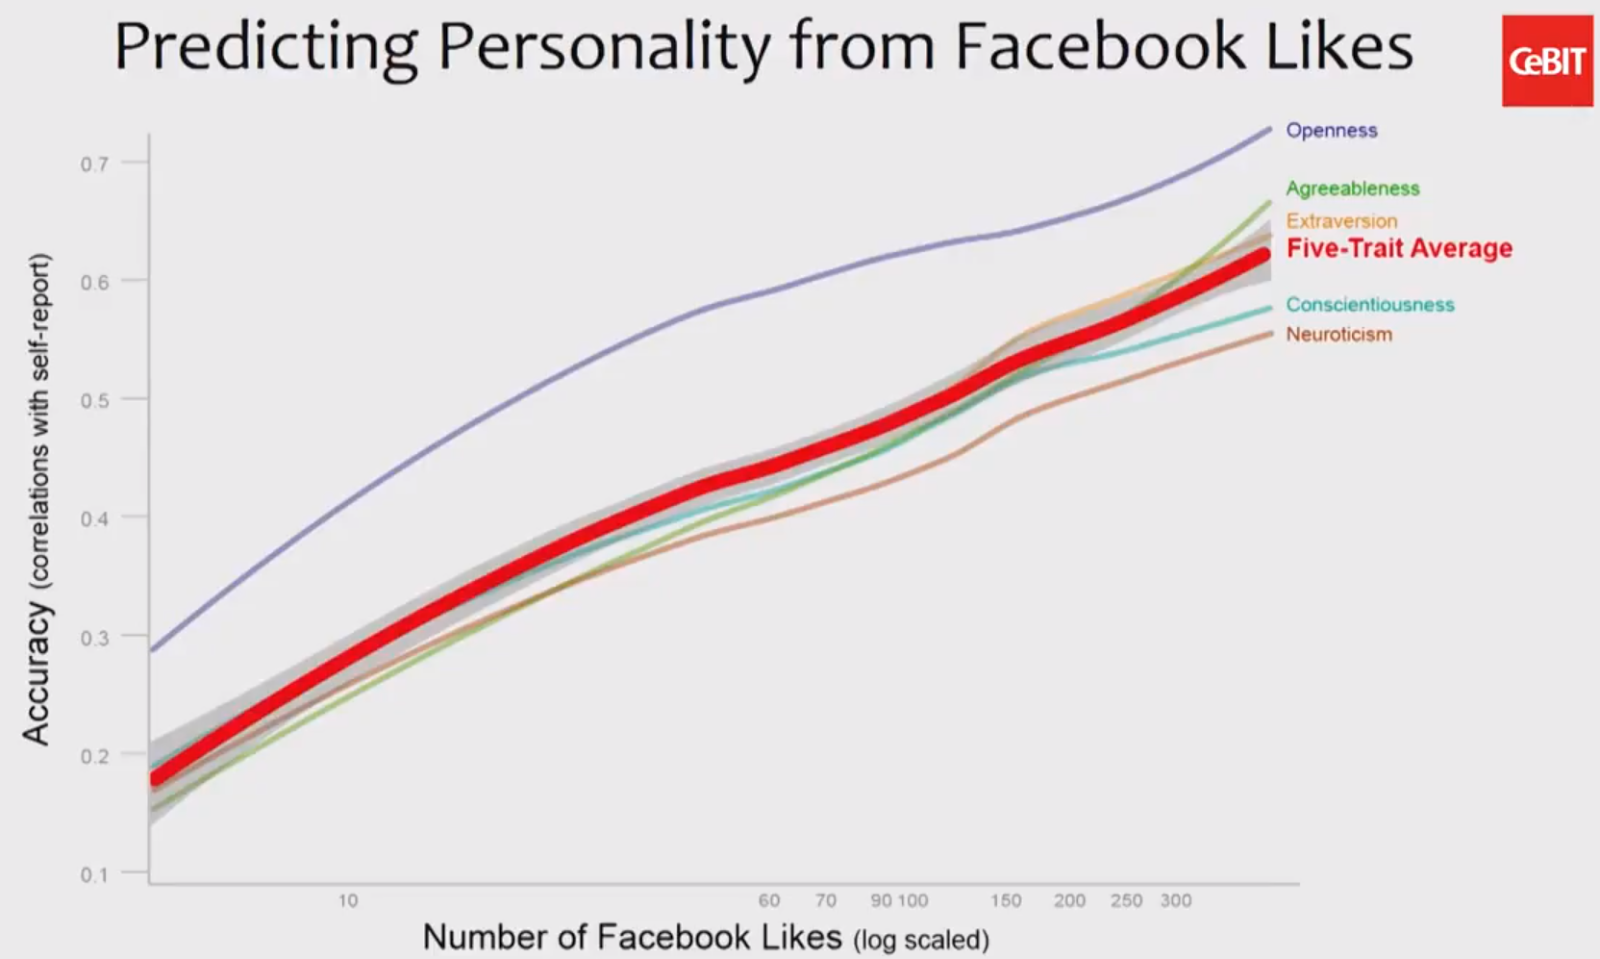
\includegraphics[width=1\textwidth]{images/analysis/talk1}
				\caption{Précision moyenne du modèle prédisant la personnalité d'un utilisateur en fonction du nombre de likes analysés\cite{kosinski-talk}.}
				\label{a-talk1}
			\end{figure}

			On remarque que la précision de la prédiction de tous les critères augmente avec le nombre de likes utilisés, ce qui n'est pas surprenant. En revanche, le tableau~\ref{a-talk-table1} montre le lien entre le nombre de likes utilisés et la précision moyenne atteinte par l'algorithme, et compare ces valeurs à la précision atteinte par d'autres êtres humains.

			\begin{table}[]
				\centering
				\begin{tabular}{lll}
					         & Précision & Nombre de likes \\
					Collègue & 0.27      & 10                            \\
					Ami      & 0.44      & 80                            \\
					Famille  & 0.5       & 100                           \\
					Epoux/se & 0.58      & 250                          
				\end{tabular}
				\caption{Précision atteinte par type de relation avec une personne, et nombre de likes nécessaires au modèle pour égaler sa précision}
				\label{a-talk-table1}
			\end{table}

			On peut voir que la précision de la prédiction de l'algorithme surpasse celle même l'époux/se d'une personne avec 250 likes, ce qui se trouve être légèrement au-dessus du nombre de likes moyen par personne, qui est de 227.

			Les possibilités de prédiction du modèle ne se limitent pas à une simple personne, et les possibilités sont nombreuses. Par exemple, Michal montre qu'il est possible de montrer une corrélation entre les visiteurs d'un certain site web, et une tendance vers certains traits psychologiques. La figure~\ref{a-talk2} montre la personnalité moyenne estimée des visitaurs du site web ```deviantart.com''' par rapport à la moyenne de tous les utilisateurs.

			\begin{figure}[ht]
				\centering
				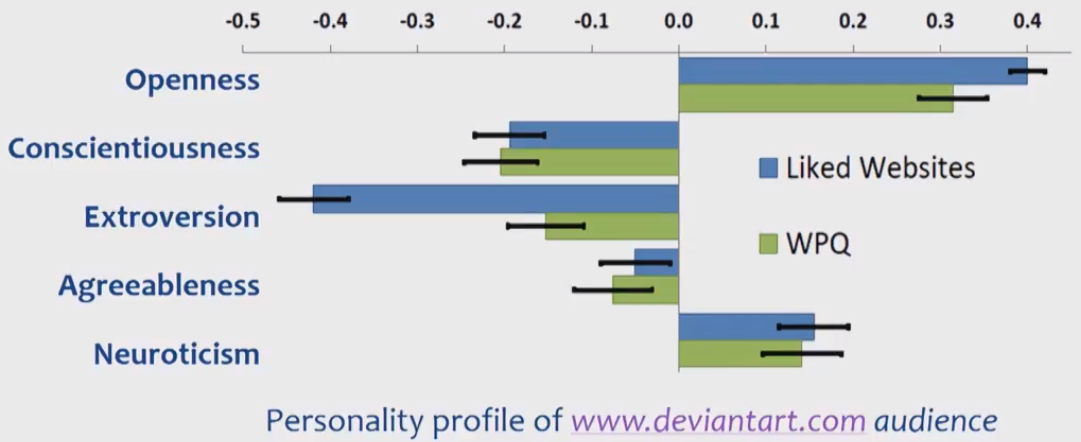
\includegraphics[width=1\textwidth]{images/analysis/talk2}
				\caption{Déviation de la personnalité moyenne estimée d'un visiteur régulier du site ```deviantart.com''' selon les cinq axes psychologiques employés\cite{kosinski-talk}.}
				\label{a-talk2}
			\end{figure}

			Ces corrélations ne sont que quelques exemples parmi un très large éventail de possibles corrélations que le modèle est capable de mettre en lumière. Les implications de telles découvertes sont massives : Il serait par exemple possible de déterminer si un utilisateur sera réceptif ou non à un certain type de publicité, par exemple. Ce genre de problématique touche à plusieurs domaines et n'est pas exactement de notre ressort ici : Des principes éthiques sont en jeu, et le sujet devient de plus en plus délicat. Mais une chose est certaine : Des likes Facebook peuvent révéler énormément d'informations.

		\subsubsection{Données}

			La quantité de données amassée par l'étude est massive. Non seulement en quantité d'utilisateurs, mais également en diversité de données. Michal Kosinski a mis en place le site web "myPersonnality Project"\cite{mypersonnality} permettant de partager cette source de données avec d'autres chercheurs. Les données comprennent, entre autres :

			\begin{itemize}
				\item Scores de personnalité selon la méthode BIG5 de >3 millions de personnes
				\item Données démographiques de >4 millions de personnes
				\item Localisation géographique de >1.5 million de personnes
				\item Vues politiques de >500'000 personnes
				\item Likes Facebook de >19 millions de personnes
			\end{itemize}

			Le type de données présenté ici n'est qu'un sous-ensemble restreint de l'ensemble des tables présentées, bien qu'il s'agisse ici des données comprenant le plus d'entrées au total.

		\subsubsection{Acquisition}

			Bien que l'objectif du site web soit de partager l'accès à cette énorme base de données, l'accès à celle-ci est loin d'être aisé. Tout d'abord, Kosinski ne met ces données à disposition que de milieux académiques, il interdit l'utilisation de ces données à des fins commerciales.

			Cependant l'accès n'est pas donné pour autant : Une demande d'accès est à lui envoyer, comprenant une présentation du projet et de ses buts par le biais d'un mail ainsi que le remplissage et l'enregistration du projet de recherche sur des sites spécialisés.

			Cette étape ne semblait constituer qu'une étape nécessiatant un temps restreint, mais un prérequis à l'envoi d'une demande d'accès à la base de données est l'approbation de l'"IRB" (Institutional Review Board), ce qui correspond à un comité d'éthique.

		\subsubsection{Conclusion}

			Etant donné les délais estimés de l'envoi de la demande à un comité d'éthique responsable puis de la demande d'accès aux données à Kosinski, nous avons écarté cette source de données de la liste principale du projet car nous n'avions pas l'assurance de disposer des données à temps pour la suite de l'étude. Bien qu'il s'agisse certainement d'un ajout conséquent aux données amassées par le projet, nous ne pouvons pas nous permettre de mettre en péril tout l'agenda du projet sur cette source de données.

	\subsection{Google Analytics et trackers}

		Etant donné que nous nous intéressons aux données des utilisateurs récupérées lors de la navigation Web, nous ne pouvons pas passer à côté de l'analyse du plus grand tracker actuel qu'est Google avec leur produit Google Analytics.

		\begin{figure}[ht]
			\centering
			
\includegraphics[width=0.4\textwidth]{images/analysis/analytics}
			\caption{Logo de la solution Google Analytics\cite{analytics}.}
			\label{a-analytics}
		\end{figure}

		Google Analytics se présente comme une solution d'analyse de statistiques d'utilisateurs dans le but d'améliorer les résultats des sites web sur lesquels il est installé. Ce produit étant totalement gratuit pour les PME, il est aujourd'hui très répandu sur le net et particulièrement en Suisse\cite{analytics-usage}.

		La figure~\ref{analytics-usage} montre la part de marché qu'occupe Google Analytics ainsi que ses compétiteurs sur les sites web Suisses.

		\begin{figure}[!h]
			\centering
			\subfloat[Utilisation de services d'analyse et de tracking\label{a-analytics-usage1}]{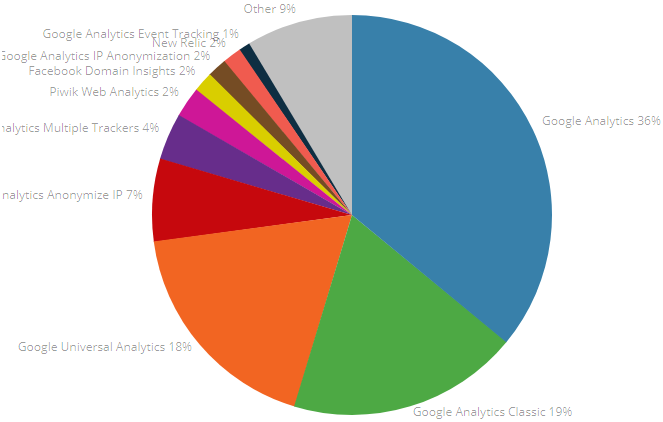
\includegraphics[width=0.45\textwidth,valign=t]{images/analysis/analytics-usage1}}
			\subfloat[Utilisation de services de mesure d'audience\label{a-analytics-usage2}]{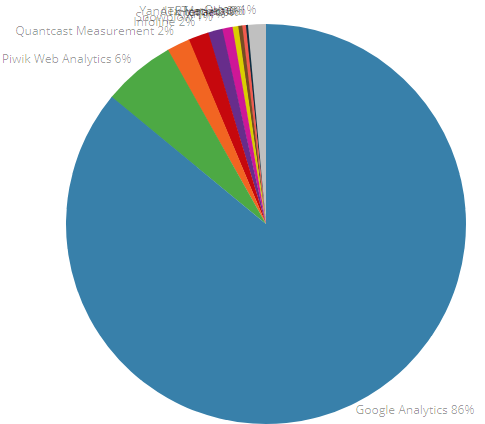
\includegraphics[width=0.45\textwidth,valign=t]{images/analysis/analytics-usage2}}
			\caption{Marché occupé par Google Analytics dans les domaines d'analyse, de tracking et de mesure d'audience sur le Web.}
			\label{analytics-usage}
		\end{figure}

		Nous pouvons calculer grâce au premier graphique que l'ensemble des produits de Google, y compris Google Analytics et ses versions proches, représentent plus de 83\% des installations de solutions dans le domaine de l'analyse et du tracking. De plus pour la sous-catégorie du marché de la mesure d'audience uniquement, Google Analytics a lui seul représente 86\% d'installations sur le Web.

		Il est donc de plus en plus évident que s'intéresser aux fonctionnalités de Google Analytics est intéressant pour les buts du projet. Nous souhaitons nous poser la question du risque encouru par les utilisateurs en se connectant sur un site web utilisant Google Analytics. Quelles informations sont prélevées ? Lesquelles sont envoyées ? Les données sont-elles anonymisées ?

	\subsection{Extensions de navigateur}